%%「論文」,「レター」,「レター(C分冊)」,「技術研究報告」などのテンプレート
%% v3.3N [2023/03/30]
%% 1. 「論文」
\documentclass[paper]{ieicej}
%\documentclass[invited]{ieicej}% 招待論文
%\documentclass[survey]{ieicej}% サーベイ論文
%\documentclass[comment]{ieicej}% 解説論文
% \usepackage[dvips]{graphicx}
\usepackage[dvipdfmx]{graphicx,xcolor}
\usepackage[fleqn]{amsmath}
\usepackage{newtxtext}% 英数字フォントの設定を変更しないでください
\usepackage[varg]{newtxmath}% % 英数字フォントの設定を変更しないでください
\usepackage{latexsym}
\usepackage{multirow}
\usepackage{url}	% \url{}コマンド用.URLを表示する際に便利
\usepackage{booktabs}

\newcommand{\todo}[1]{\colorbox{yellow}{{\bf TODO}:}{\color{red} {\textbf{[#1]}}}}

\setcounter{page}{1}

\field{}
\jtitle{複数のソフトウェア変更履歴データの統合によるコーディング規約違反の修正予測精度の評価}
\etitle{Evaluating Coding Convention Violation Fix Prediction Accuracy Based on Code Features Across Multiple Projects}
\authorlist{%
 \authorentry{亀岡 令}{Ryo Kameoka}{jibun}\MembershipNumber{}
 \authorentry{伊原 彰紀}{Akinori Ihara}{teacher}\MembershipNumber{}
 %\authorentry{和文著者名}{英文著者名}{所属ラベル}\MembershipNumber{}
 %\authorentry[メールアドレス]{和文著者名}{英文著者名}{所属ラベル}\MembershipNumber{}
 %\authorentry{和文著者名}{英文著者名}{所属ラベル}[現在の所属ラベル]\MembershipNumber{}
}
\affiliate[jibun]{和歌山大学システム工学研究科}{Wakayama university}
\affiliate[teacher]{和歌山大学}{Wakayama university}
%\affiliate[所属ラベル]{和文所属}{英文所属}
%\paffiliate[]{}
%\paffiliate[現在の所属ラベル]{和文所属}
\jalcdoi{???????????}% ← このままにしておいてください

\begin{document}
\begin{abstract}
% \todo{最後に書く}
OSS開発では,可読性の高いソースコードが重要であり,コーディング規約はそのための手段となる.しかし,規約違反コードは大量に検出されるため,修正は一部に留まることが多い.従来研究では,プロジェクト自身の修正履歴に基づき違反箇所の修正優先度を予測してきたが,予測精度が十分でない場合が多い.本研究では,他の複数プロジェクトの開発履歴を学習させることによる予測精度の変化を検証し,予測精度が向上する条件について分析する.
\end{abstract}
\begin{keyword}
静的解析, 機械学習, 可読性
\end{keyword}
\begin{eabstract}
In OSS development, readable code is vital, and coding conventions help achieve this. Static analysis detects many violations, but only some are fixed. Prior work predicts fix priority using a project's history. This study examines how learning from other projects' histories affects the accuracy of predicting which violations get fixed. It also analyzes prediction differences between this approach and prior methods in projects with significant accuracy changes.
\end{eabstract}
\begin{ekeyword}
%英文キーワード
\end{ekeyword}
\maketitle

\section{まえがき}
% \todo{最後に書く}
コーディング規約とは,ソースコードを一定の品質に保つための記述方法について,禁止事項や推奨事項を定め,保守性を高めるためのコーディングスタイルなどをまとめたものである.
ソフトウェア開発者はコーディングスタイルの共通化や,ソースコードの最適化のためにコーディング規約を遵守することで,可読性の高いソースコードを書くことができる\cite{EffectsSAT}.また,プロジェクトへのコーディング規約の導入によって,ソースコードの理解の促進やバグの早期発見などへの効果も確認されている\cite{Beller2}\cite{Johnson}\cite{Beller}.

コーディング規約に違反している箇所を機械的に検出するために静的解析ツールが用いられる.
静的解析ツールはソースコードを実行することなく,ソースコードに含まれるコーディング規約に違反している箇所を検出することができ,継続的インテグレーションのプロセスの1つとして使用されることも多い.
静的解析ツールは,ソースコード中のコーディング規約に違反しているコード断片を正規表現などにより検出することができ,開発者は静的解析ツールが検出した違反を確認することで,コーディング規約に違反している箇所を速やかに修正することができる.
静的解析ツールは多くの規約の種類を定義しているため,修正の必要がないような軽微な違反を含む大量の規約違反検出結果が出力されることが頻繁に発生する.静的解析ツールの大量の検出結果は開発効率の低下につながるため,修正が必要な違反を検出するための研究が行われている\cite{Nguyen}.

従来研究では大量に検出されるコーディング規約違反の中から,優先して修正すべき違反を検出する手法が数多く提案されている\cite{JyuraiPre}
% % \todo{引用増やせれば}.
他にも静的解析ツールの検出結果を優先度づけする研究は数多く行われている.
従来研究の多くは,単一プロジェクトの規約違反修正履歴を学習することで各プロジェクトのコーディングの慣習を捉えた予測を行っているが,予測精度が十分でない.その原因の一つとして,学習データのスパース性が考えられる.学習データ数自体は十分でも正例数が少なく,学習が十分できないことが考えられる.
Tabassumらは,不具合予測やソースコードの自動修正において,データ不足,コールドスタート問題への対応として,異なるプロジェクトの開発データを用いることによって学習データを補う手法を提案しているが,不具合予測であり,コーディング規約違反に関する研究は行われていない\cite{Tabassum}.
異なるプロジェクトのデータを用いることで,コールドスタート問題への対処は可能であるが,実装方針の異なるプロジェクトのデータを学習することとなるため,十分なデータがある場合には,単一プロジェクトのデータのみを学習したほうが高い予測精度を得ることができる.

本研究では,複数プロジェクトの開発データを予測モデルの学習に使用することによる,コーディング規約違反の修正予測精度への影響を明らかにする.
提案手法として2種類の予測モデルを構築する.1つは,複数プロジェクトのデータを単純に結合し,学習する全学習手法である.
もう1つは,複数プロジェクトのデータを統合する際に,類似するプロジェクトに絞り,統合し学習する選定学習手法である.
本研究の提案手法は,著者らが過去に提案した手法から,類似したプロジェクトのみを学習データに統合する選定学習を新たに提案している\cite{mine}\cite{mine_live}.選定学習の結果として,一部プロジェクトにおいて,再現率の大幅な改善が見られた.
% また,本研究では先行研究では行っていなかった予測結果の詳細な分析まで行っている.

本研究の貢献として,静的解析ツールの結果から修正すべき違反のみを正確に推薦することができれば,必要修正箇所のみをLLMなどを用いたコードの自動修正を行うことが可能となり,コードの品質を高く保つことが容易になる.

続く\ref{chap:background}章では,コーディング規約違反の検出と,従来研究について述べ,\ref{chap:approach}章では本研究における実験の全体像と提案手法について述べる.\ref{chap:result}章では,評価結果を示し,\ref{chap:consideration}章では考察を述べる.\ref{chap:heuristic}章では本研究の妥当性への脅威について述べ,\ref{chap:end}章でまとめる.

\section{コーディング規約と規約違反の検出}\label{chap:background}

\subsection{コーディング規約違反}

コーディング規約とは,オープンソースソフトウェア開発や開発チームのような複数人でソフトウェア開発を行う際に,プログラミングにおける記述方法についてまとめたものである.
規約の中には変数やクラスなどの命名規則について定めたものや,関数の長さや複雑度の上限のようなソースコードの可読性に関するルールや,エラーの原因となる部分の検出,その他禁止事項,制限事項,推奨事項などが定義されている.
コーディング規約は,プログラミングに関するルールが幅広く定められており,プログラミング言語ごとに複数存在している.例えばPython言語のPEP8,Java言語のCode Conventions for the Java Programming LanguageやGoogle Java Style Guide,JavaScript言語のGoogle JavaScript Style GuideやAirbnb JavaScript Style Guideのようにプログラミング言語ごとに違反の`種類'や`基準'が異なる規約が複数存在する.

コーディング規約への違反の検出は基本的に,静的解析ツールが用いられる.静的解析ツールにも各言語ごとに複数の種類があり,参照している規約の種類や,違反を検出した際のメッセージのフォーマット,検出する違反のカスタマイズ性の高さなどが異なる.
開発者は静的解析ツールを継続的インテグレーションツールとして利用することで,開発の生産性を向上させることができる.
ソースコードの品質を良い状態で保つことは重要であり,品質の悪いコードは,品質の良いコードに比べて15倍の欠陥が含まれることを明らかにしている\cite{静的解析ツールの効果}.

静的解析ツールは各違反ごとに定められたルールに合致した場合にすべて違反として検出し出力するため,大量の検出結果が出力されることが頻繁に発生する.実際に多くのプロジェクトで,静的解析ツールが大量の規約違反を検出することが多いことを従来研究で明らかにしている\cite{UsingStaticAnalysisTools2}.
大量の違反の検出結果には修正する必要がないような軽微な違反も含まれ,それらを開発者がレビューし保守するには多くのコストを要するため困難である.
さらに様々な違反から優先して修正すべき規約違反を特定することは,開発の経験や,複雑なソースコードの理解が必要であるため,プロジェクト開発において容易でない\cite{shuseisarenai}.


\subsection{従来研究}

従来研究では静的解析ツールの修正する必要のない違反を含む大量の検出結果によって開発効率の低下を防ぐため,Ruthruffらは機械学習モデルを用いて優先して修正すべき違反を特定する手法を提案している\cite{JyuraiPre}.
Kimらは静的解析ツールの出力結果をベイジアンネットワークに活用することにより,コーディング規約に違反しているコードの修正優先度の予測を行う手法を提案している\cite{beizu}.
これらの研究のほかにも静的解析ツールによって検出された規約に違反しているコードの修正優先度付けを行う研究や,修正の要否を予測する研究は数多く行われている\cite{Wang}\cite{Qing}\cite{HowFar}.
機械学習のモデル構築には,規約違反コードの修正優先度予測対象のプロジェクトの過去の規約違反修正履歴を学習データとし,新しいデータを評価用データとすることで構築したモデルの評価を行っている.

従来手法では,予測対象とするプロジェクトの過去の規約違反修正履歴を学習データとして,予測モデルを構築している.各プロジェクトにはコーディングスタイルなどが存在し,修正の要否はプロジェクトごとに異なるため,評価用データと同じプロジェクトのデータを学習するほうが,他プロジェクトのデータを学習するより高い予測精度が得られると考えられる.
しかし,評価用データと同じプロジェクトを学習データとする場合,出現する規約違反の種類や,各違反の修正率が大きく異なる\cite{Panichella}.そのため,規約違反が修正される(正例)と修正されない(負例)の数が不均衡になる場合や,データサイズが小さいことにより,十分な学習ができず予測精度が低下することが示唆される.

本研究では,予測モデルの構築の際に用いる学習データに評価用データとは異なる別プロジェクトの規約違反修正履歴を用いることによる,規約違反コードの修正要否の予測精度への影響を明らかにする.
名倉らは,複数プロジェクトを用いてコーディング規約違反の発生の増減の予測を行っているが,発生した違反が修正されるか否かを予測することは行っていないため,予測の点において本研究との差分となっている\cite{nagura}.
複数プロジェクトの修正履歴データを用いて学習データサイズの拡張を図ることにより,予測精度の向上を期待できるが,他プロジェクトで修正される規約が予測精度の向上に寄与するとは限らない.
そこで,本研究では複数プロジェクトの開発データを学習した場合の予測精度への影響を明らかにすることを目的とする.

\section{コーディング規約違反の修正要否予測モデルの構築手法}\label{chap:approach}
%%%%%%%%%%%%%%%%%%%%%%%%%%%

\subsection{概要}

\begin{figure*}[t]
	\centering
	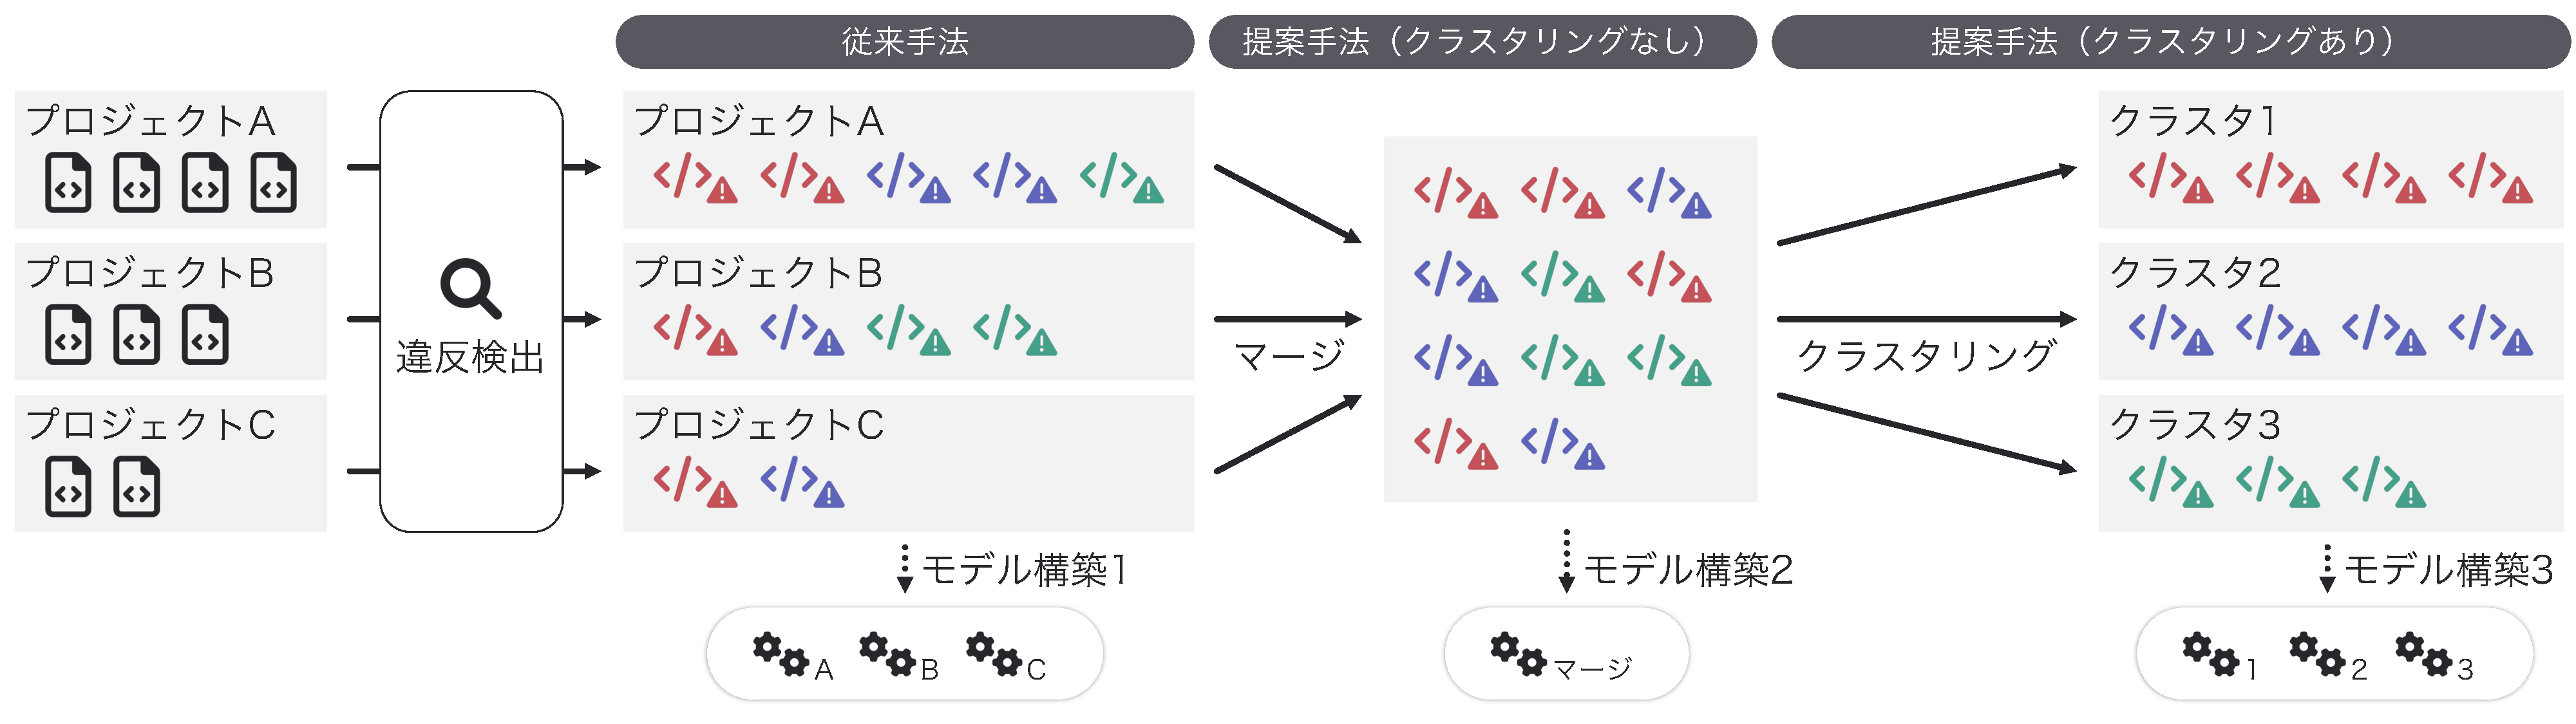
\includegraphics[width=0.8\linewidth]{fig/kameoka_fig1.pdf}
	\caption{\todo{1図の更新}}
	\label{fig:Teiannsyuhou}
\end{figure*}

% \todo{図の更新}図\ref{fig:Teiannsyuhou}は本研究の提案手法を評価するための検証手法を示す.本研究では,静的解析ツールによって検出されたコーディング規約違反を修正すべき違反かそうでない違反かの2値に分類する機械学習モデルを3種類作成する.
\todo{図の更新}図\ref{fig:Teiannsyuhou}に本研究における機械学習モデルの構築と評価の概要を示す.本研究では,静的解析ツールによって検出されたコーディング規約違反を修正が必要な違反かそうでない違反かの2値に分類する機械学習モデルを3種類作成する.

\begin{enumerate}
  \item 単一学習(従来手法):従来研究の手法を採用したモデルであり,予測対象のプロジェクトの過去の規約違反修正履歴のみを学習する予測モデルを構築\cite{JyuraiPre}
  \item 全学習(提案手法):複数プロジェクトの規約違反修正履歴を学習させる手法で,すべてのプロジェクトの学習データを結合し,学習する予測モデルを構築
  \item 選定学習(提案手法):複数プロジェクトの規約違反修正履歴を学習させるが,予測対象プロジェクトと規約違反の修正傾向の似たものだけを学習する予測モデルを構築
\end{enumerate}

全学習では,データセット内のすべてのプロジェクトのデータを学習する.そのため,プロジェクトごとのコーディングスタイルを無視した学習を行う.コーディングスタイルの異なるプロジェクトのデータは学習のノイズとなり,予測精度が低下する恐れがある.しかし,規約違反の修正予測の分野において複数プロジェクトのデータを学習に用いる手法は提案されていないため,全学習の評価が必要である.

選定学習において,予測対象のプロジェクトと規約違反の修正傾向の類似したプロジェクトのみを学習させる理由は,学習させるデータとして不適切なデータを取り除くためである.全学習で懸念点としてあげたように,単純に全てのプロジェクトの修正履歴のデータを学習させた場合,予測対象のプロジェクトとは異なる修正傾向をしているデータを学習することが考えられる.そのため,予測対象以外の修正履歴を学習データに使用するには,ノイズとなるデータを削減するため修正傾向の似たプロジェクトのデータのみを利用する必要がある.
また,選定学習では,コーディング規約違反の修正傾向の似たプロジェクトのみを収集するために類似度の測定を行っている.類似度の測定時に,欠損値補完を用いる方法と,用いない方法の2種類を検証する.



モデル(1)から(3)を構築,予測結果の評価を行うことで,コーディング規約違反の修正要否予測における,複数プロジェクトを学習に用いることの有効性を明らかにする.




\subsection{学習プロジェクトの選定方法} \label{chap:選定方法}

全学習,選定学習の予測モデル構築時に学習データとして予測対象以外のプロジェクトのデータも学習に使用する.全学習ではデータセット内のプロジェクトのすべてのデータを学習する.
選定学習では,複数プロジェクトのデータを学習に利用するにあたって,学習データとしてノイズとなってしまうデータを削減するために,予測対象プロジェクトとコーディング規約違反の修正傾向が類似したプロジェクトのみを学習に使用する.
プロジェクト間の類似度の測定には,コーディング規約違反の修正率に着目する.修正率は式(\ref{eq:fixrate})のように計算する.この修正率をプロジェクトごとに,コーディング規約違反IDごとに算出する.
算出した修正率をもとに,ジャッカード係数とユークリッド距離の二種類の類似度を測定し,それぞれに閾値を設け,一定の類似度以上のプロジェクトのみを選定する.
また,ユークリッド距離の測定時に,違反が一度も発生していないコーディング規約については修正率がnullとなるので,nullのままではユークリッド距離は測定できない.そこで,選定学習の類似度の測定方法として,ユークリッド距離の測定時にnullを計算から省く方法と,nullをプロジェクトの平均修正率で欠損値補完してユークリッド距離を計算する二種類のユークリッド距離の測定を行い,それぞれの結果を評価する.
欠損値の補完には,最大値,最小値,ゼロなど,さまざまな手法が存在する.本研究では,一度も検出されなかった違反の修正率を補完するため,欠損値をゼロで補完すると,その違反が全く修正されなかったという意味になる.そのため,本研究では当該プロジェクトの平均値で補完を行う.
\todo{表を入れるかは検討}

2種類の類似度の測定により,プロジェクト間のコーディング規約の修正傾向の類似度の測定が可能であるが,統合した学習データに利用するプロジェクトを決定するための類似度の最適な閾値については不明である.
よって本研究では,それぞれの閾値を段階的に変化させ,最も予測精度の良い閾値を採用する.検証する範囲としては,ジャッカード係数を0.1以下から0.5以下までを0.1ずつ変化させ,ユークリッド距離は1.5以下から5.0以下までを0.5ずつ変化させこれらの組み合わせを網羅的に検証する.それぞれの閾値の最小値と最大値は,その値以降では全てのプロジェクト該当する,もしくは該当プロジェクトが一つもなくなる境界値になっている.

\begin{equation}
\label{eq:fixrate}
\text{修正率} = \frac{\text{違反の修正された数}}{\text{違反の発生した数}}
\end{equation}





\subsection{説明変数・目的変数の計測方法}


%-------------------------
\begin{figure}[t]
	\centering
	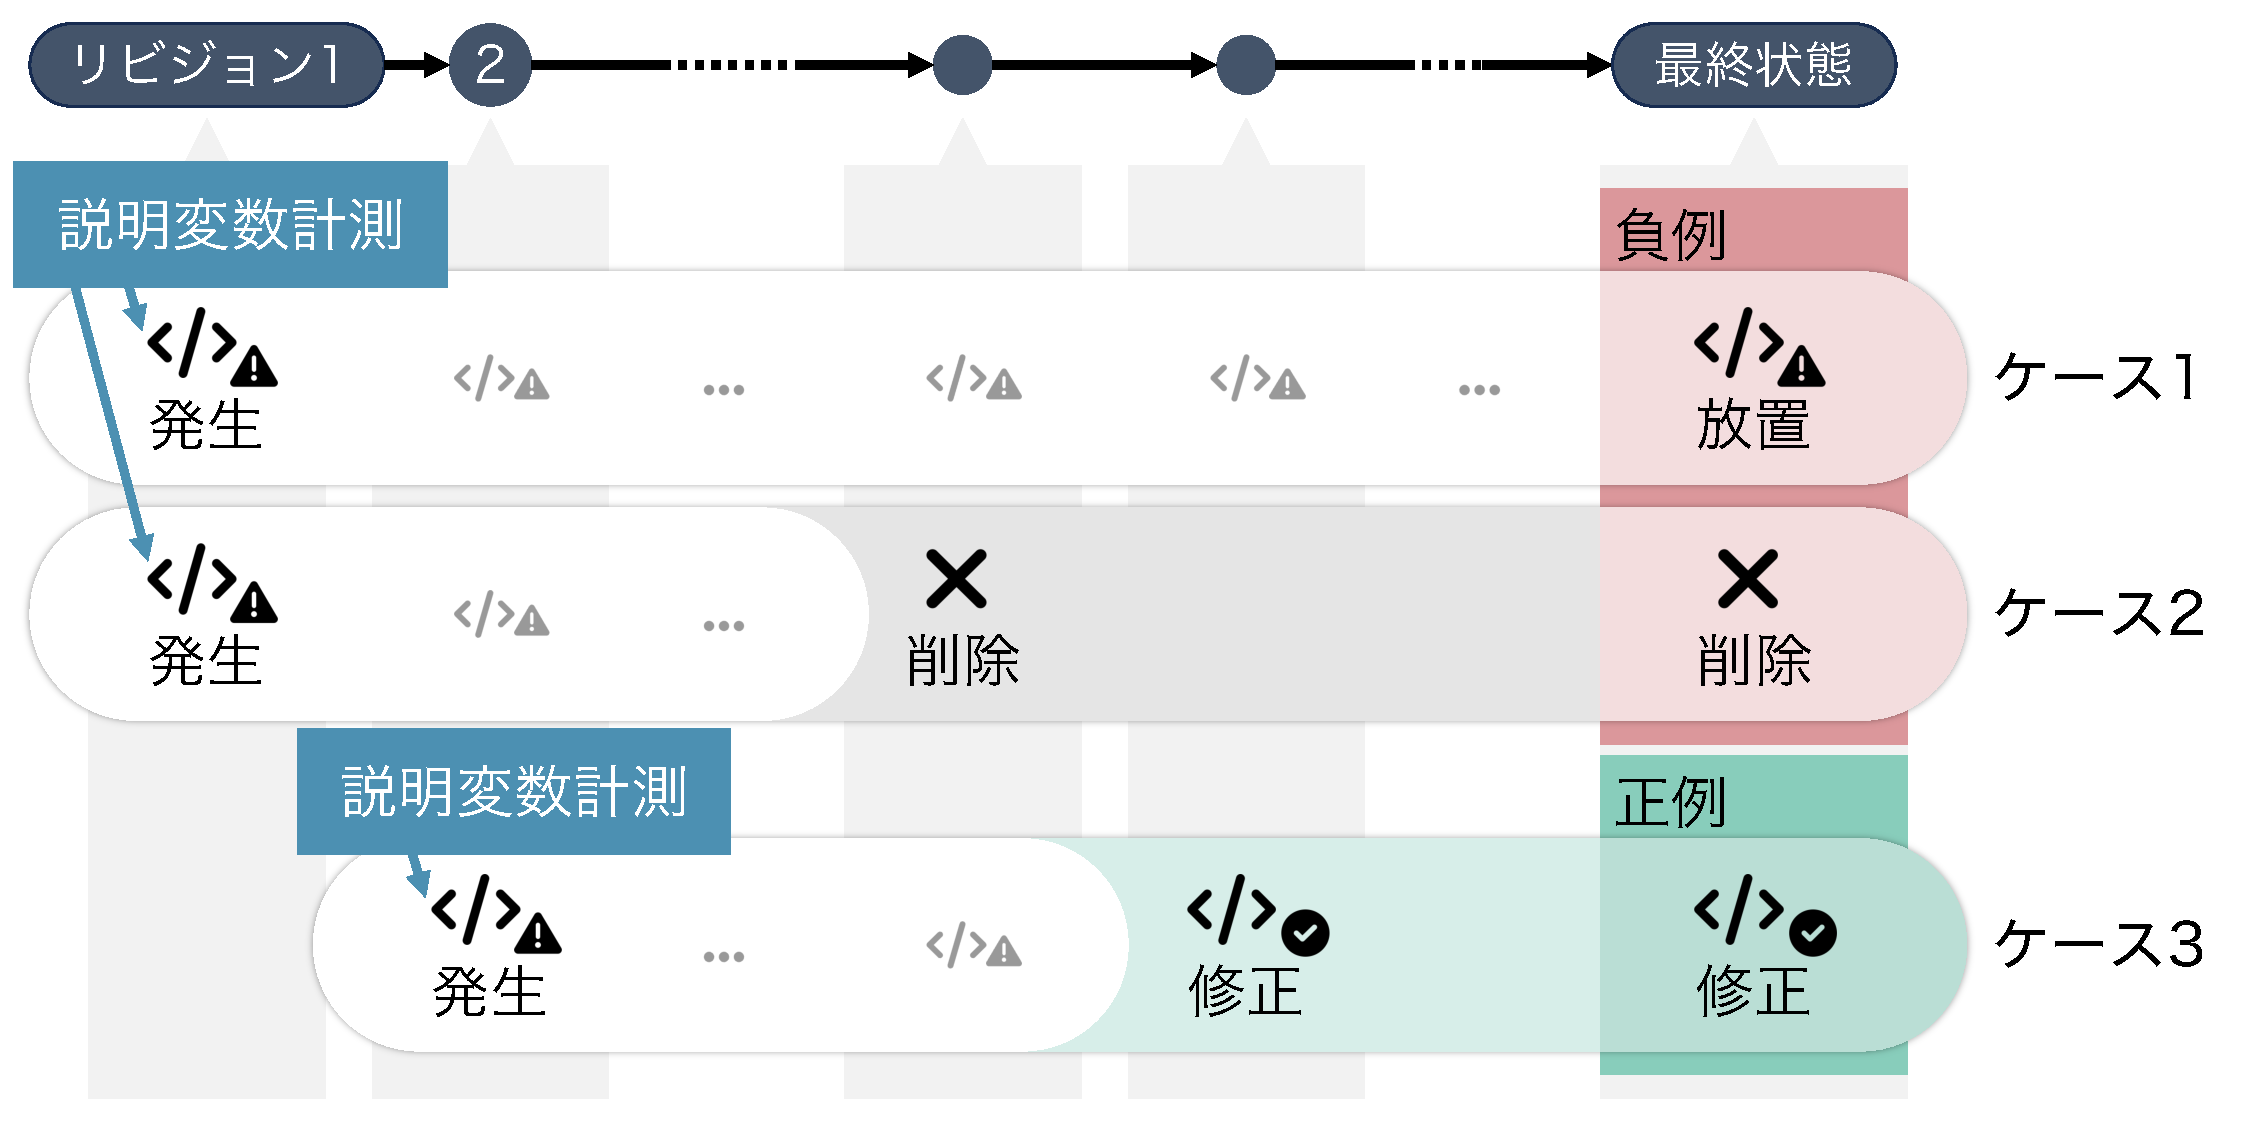
\includegraphics[width=1.0\linewidth]{fig/kameoka_fig2.pdf}
    % \includegraphics[width=0.25\textwidth, bb=0 0 4 3]{fig/fig2.pdf}
	\caption{説明変数と目的変数の計測方法}
	\label{fig:mokutekihensu}
\end{figure}
%-------------------------

図\ref{fig:mokutekihensu}に本研究における説明変数と目的変数の計測位置と,計測方法を示す.本研究では,規約違反の修正履歴から静的解析ツールによって初めて違反が検出された場所を説明変数の計測地点とし,違反コードの最終状態によって,目的変数を計測する.
目的変数の計測についてケースごとにまとめたものが表\ref{tab:pos_neg}である.
図\ref{fig:mokutekihensu}と表\ref{tab:pos_neg}に示すケース1からケース3はそれぞれ対応する同じ事象を示す.
説明変数は,ソースコードの特徴量であるコード行数,コメント行数,循環的複雑度などを含むソースコードに関する特徴量43種類に,コーディング規約違反IDをOne-hotベクトル化したものを加えた合計44種類の特徴量を使用する.ソースコードの特徴量の取得にはテクマトリックス株式会社が開発する静的解析ツールUnderstandを用いて計測する.

%----------------------
\begin{table}[t]
    \centering
    \caption{正例と負例の分類}
    \label{tab:pos_neg}
    \scalebox{0.85}{
    \begin{tabular}{l|l}
         \hline
            分類 & 説明\\ \hline
            負例(ケース1) & コーディング規約の違反が放置されているコード断片\\
            負例(ケース2) & コーディング規約に違反していたコード断片が削除された\\
            正例(ケース3) & コーディング規約に違反していたコード断片が修正された\\
         \hline
    \end{tabular}
    }
\end{table}
%-----------------------

\subsection{機械学習モデルの構築と評価}

本研究で利用する予測アルゴリズムは,離散値を利用する2値分類に協力なRandomForestを用いる.
従来の研究でも明らかにされているように,コーディング規約違反の修正に関するデータは,違反が修正された正例が少なく,修正されない負例が多い不均衡なデータであるため,各予測モデルを構築するためのPythonパッケージに用意されているオプションであるclass\_weightsを用いることによって,2クラスデータに重みづけを行う.
また,学習の反復回数を定めるイテレーション回数を10,000に設定する.


\subsection{データセット}

% \begin{figure}[t]
% 	\centering
%     % 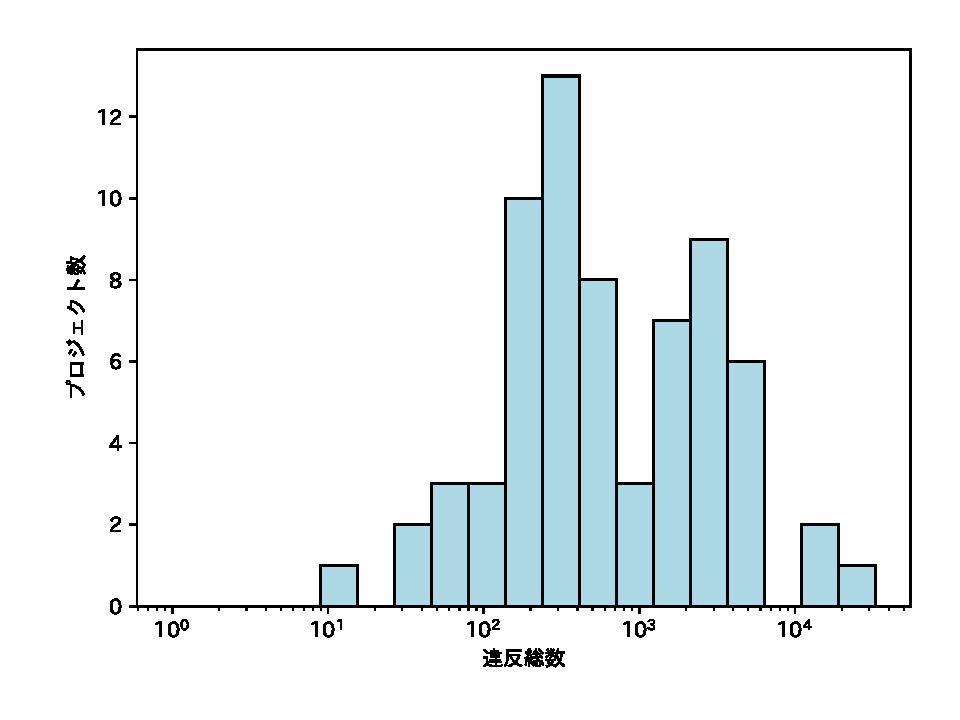
\includegraphics[width=0.25\textwidth, bb=0 0 4 3]{fig/dataset_hist.pdf}
% 	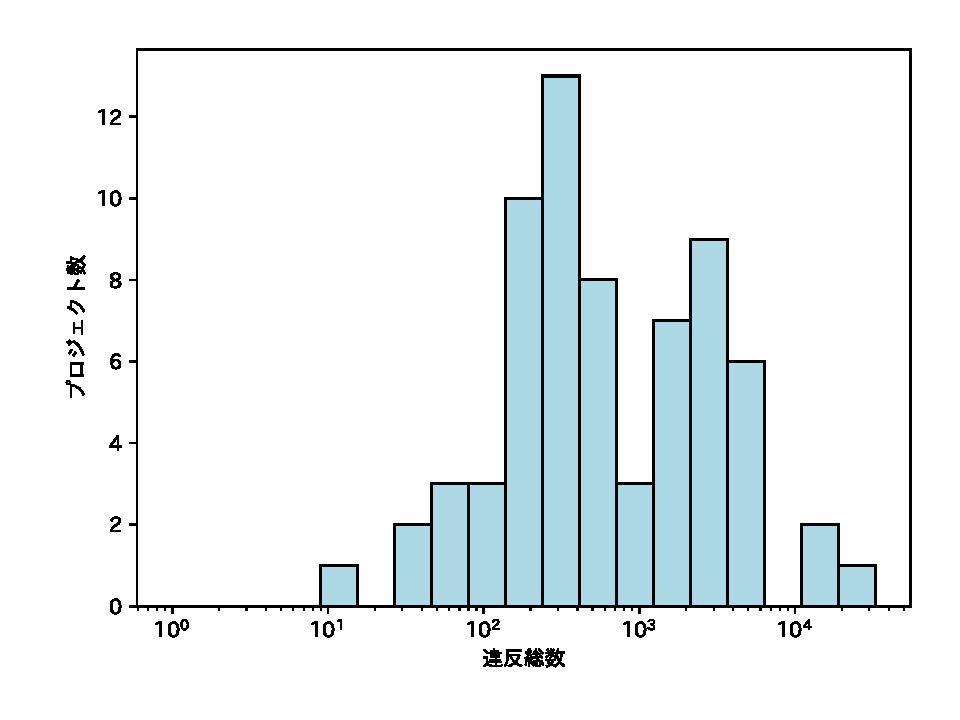
\includegraphics[width=1\linewidth]{fig/dataset_hist.pdf}
% 	\caption{データセットに含まれるプロジェクトごとの違反総数のヒストグラム}
% 	\label{fig:dataset}
% \end{figure}

\begin{table}[t]
    \centering
    \caption{データセット統計量}
    \label{tab:dataset_statistics}
    \begin{tabular}{ccc}
        \toprule
        総データ平均値 & 正例数平均値 & 負例数平均値 \\
        \midrule
        4,465 & 1,147 & 3,318 \\
        \bottomrule
    \end{tabular}
\end{table}


本研究ではケーススタディとして,OSSライブラリ検索サービスであるLibraries.io\footnote{Libraries.io: \url{https://libraries.io/}}からPython言語で実装され,静的解析ツールPylintを開発に使用しており,GitHubにソフトウェア,および規約違反修正履歴を公開しているプロジェクトを対象とする.
特に,Libraries.ioにおいてOSSの人気度合いや活発度合いを示すSourceRankの上位1,500プロジェクトから静的解析ツールの設定ファイル(pylintrc,または.pylintrc)を保有するプロジェクトの内,取得した目的変数を学習用データと検証用データに分割した際に,どちらのデータにも正例と負例を含む20プロジェクトを対象とする.
各分析対象プロジェクトにおいて,2018年12月から1,000日間のコミット履歴を分析対象とする.

実験対象のプログラミング言語としてPythonを選択した理由は,機械学習やデータ分析の需要が年々重要となってきており,Pythonは豊富なライブラリや簡潔な記述ができることから,需要が高くいからである.
また,複雑なプログラムを書くにあたり,可読性は重要な指標であり従来研究では,JavaやC言語を分析対象としているものが多く,Python言語はこの分野の予測対象とされていないためPythonを実験対象の言語とした.

表\ref{tab:dataset_statistics}にデータセットの統計量を示す.表からわかるように負例数が正例数の約3倍となっており,スパース性が高いことがわかる.

%%%%%%%%%%%%%%%%%%%%%%%%%%%
\section{評価実験}\label{chap:result}
%%%%%%%%%%%%%%%%%%%%%%%%%%%



% \subsection{実験結果}
\subsection{複数プロジェクトのデータを学習に利用することで予測精度はどのように変化するか?}

\begin{table*}[t]
  \centering
  \caption{手法ごとの予測結果}
  \label{table:result1}
  \resizebox{\textwidth}{!}{%
  \begin{tabular}{lcccccccccccc}
    \toprule
    \multirow{2}{*}{プロジェクト名} 
    & \multicolumn{3}{c}{単一学習} 
    & \multicolumn{3}{c}{全学習} 
    & \multicolumn{3}{c}{選定学習} 
    & \multicolumn{3}{c}{\shortstack{選定学習\\(欠損値補完あり)}} \\
    \cmidrule(lr){2-4} \cmidrule(lr){5-7} \cmidrule(lr){8-10} \cmidrule(lr){11-13}
    & 適合率 & 再現率 & F1値 & 適合率 & 再現率 & F1値 & 適合率 & 再現率 & F1値 & 適合率 & 再現率 & F1値 \\
    \midrule
        sockeye & 0.75 & \textbf{\underline{0.83}} & \textbf{\underline{0.79}} & 0.75 & 0.81 & 0.78 & \textbf{\underline{0.77}} & 0.82 & 0.79 & 0.75 & \textbf{\underline{0.83}} & \textbf{\underline{0.79}} \\
        coretools & 0.14 & 0.24 & 0.18 & 0.07 & 0.39 & 0.12 & 0.05 & 0.07 & 0.06 & 0.14 & 0.24 & 0.18 \\
        \underline{howdoi} & 0.78 & 0.99 & 0.87 & 0.07 & 0.97 & 0.13 & 0.72 & 0.99 & 0.84 & 0.72 & 0.99 & 0.84 \\
        schema\_salad & 0.66 & 0.58 & 0.62 & 0.59 & 0.22 & 0.32 & 0.66 & 0.36 & 0.47 & 0.66 & 0.58 & 0.62 \\
        serverless-application-model & 0.72 & 0.27 & 0.39 & 0.74 & 0.20 & 0.32 & 0.77 & 0.32 & 0.45 & 0.72 & 0.27 & 0.39 \\
        SoCo & 0.67 & 0.64 & 0.66 & 0.74 & 0.54 & 0.62 & 0.70 & 0.61 & 0.65 & 0.67 & 0.64 & 0.66 \\
        behave & 0.33 & 0.37 & 0.35 & 0.26 & 0.35 & 0.30 & 0.33 & 0.24 & 0.28 & 0.33 & 0.37 & 0.35 \\
        OWSLib & 0.61 & 0.77 & 0.68 & 0.63 & 0.77 & 0.69 & 0.62 & 0.77 & 0.68 & 0.61 & 0.77 & 0.68 \\
        pynput & 0.34 & 0.87 & 0.49 & 0.47 & 0.54 & 0.50 & 0.31 & 0.75 & 0.44 & 0.34 & 0.87 & 0.49 \\
        schematics & 0.44 & 0.75 & 0.55 & 0.45 & 0.77 & 0.57 & 0.45 & 0.74 & 0.56 & 0.44 & 0.75 & 0.55 \\
        \underline{hickle} & 0.14 & 0.14 & 0.14 & 0.24 & 0.53 & 0.33 & 0.24 & 0.55 & 0.33 & 0.13 & 0.17 & 0.15 \\
        \underline{python-sdk} & 0.43 & 0.45 & 0.44 & 0.31 & 0.63 & 0.41 & 0.44 & 0.71 & 0.54 & 0.43 & 0.63 & 0.51 \\
        rtv & 0.73 & 0.51 & 0.60 & 0.62 & 0.33 & 0.43 & 0.71 & 0.51 & 0.60 & 0.73 & 0.51 & 0.60 \\
        datadogpy & 0.02 & 0.05 & 0.03 & 0.13 & 0.46 & 0.20 & 0.12 & 0.33 & 0.17 & 0.02 & 0.05 & 0.03 \\
        pychromecast & 0.93 & 0.89 & 0.91 & 0.87 & 0.75 & 0.81 & 0.90 & 0.88 & 0.89 & 0.93 & 0.89 & 0.91 \\
        \underline{pyscard} & 0.08 & 0.17 & 0.11 & 0.07 & 0.50 & 0.12 & 0.06 & 0.33 & 0.10 & 0.12 & 0.33 & 0.18 \\
        imgaug & 0.10 & 0.05 & 0.07 & 0.50 & 0.02 & 0.03 & 0.10 & 0.05 & 0.07 & 0.10 & 0.05 & 0.07 \\
        \underline{GPflow} & 0.64 & 0.89 & 0.74 & 0.61 & 0.18 & 0.28 & 0.64 & 0.82 & 0.72 & 0.65 & 0.90 & 0.75 \\
        \underline{transitions} & 0.83 & 0.96 & 0.89 & 0.82 & 0.98 & 0.89 & 0.81 & 0.98 & 0.89 & 0.84 & 0.96 & 0.89 \\
        pyphi & 0.67 & 0.78 & 0.72 & 0.69 & 0.92 & 0.79 & 0.67 & 0.78 & 0.72 & 0.67 & 0.78 & 0.72 \\
    \bottomrule
  \end{tabular}
  }
\end{table*}


\begin{figure}[t]
	\centering
        % 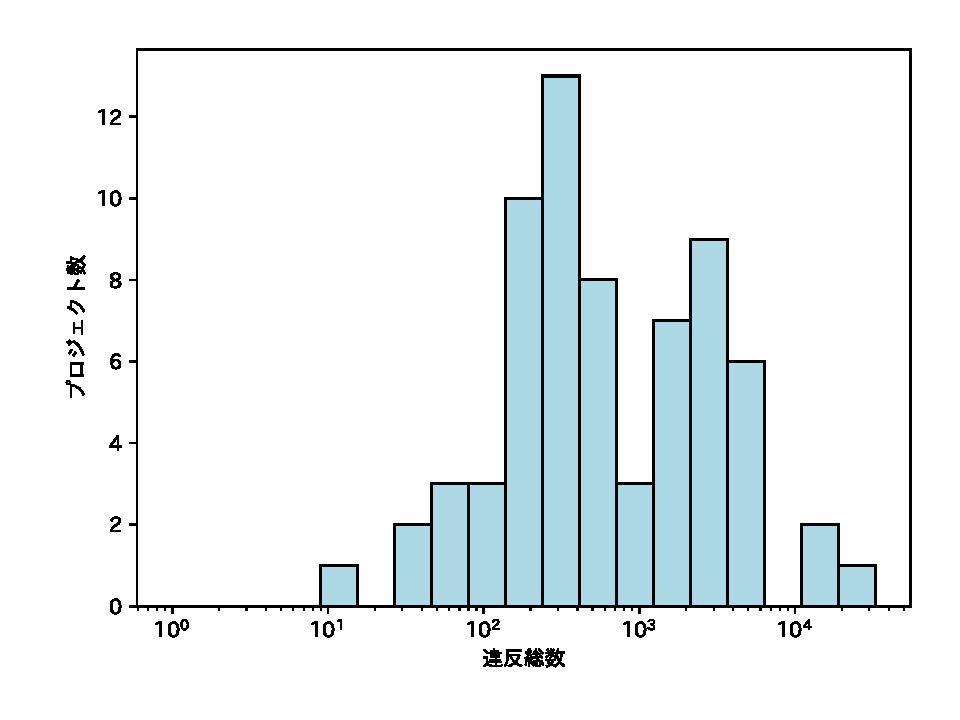
\includegraphics[width=0.25\textwidth, bb=0 0 4 3]{fig/dataset_hist.pdf}
	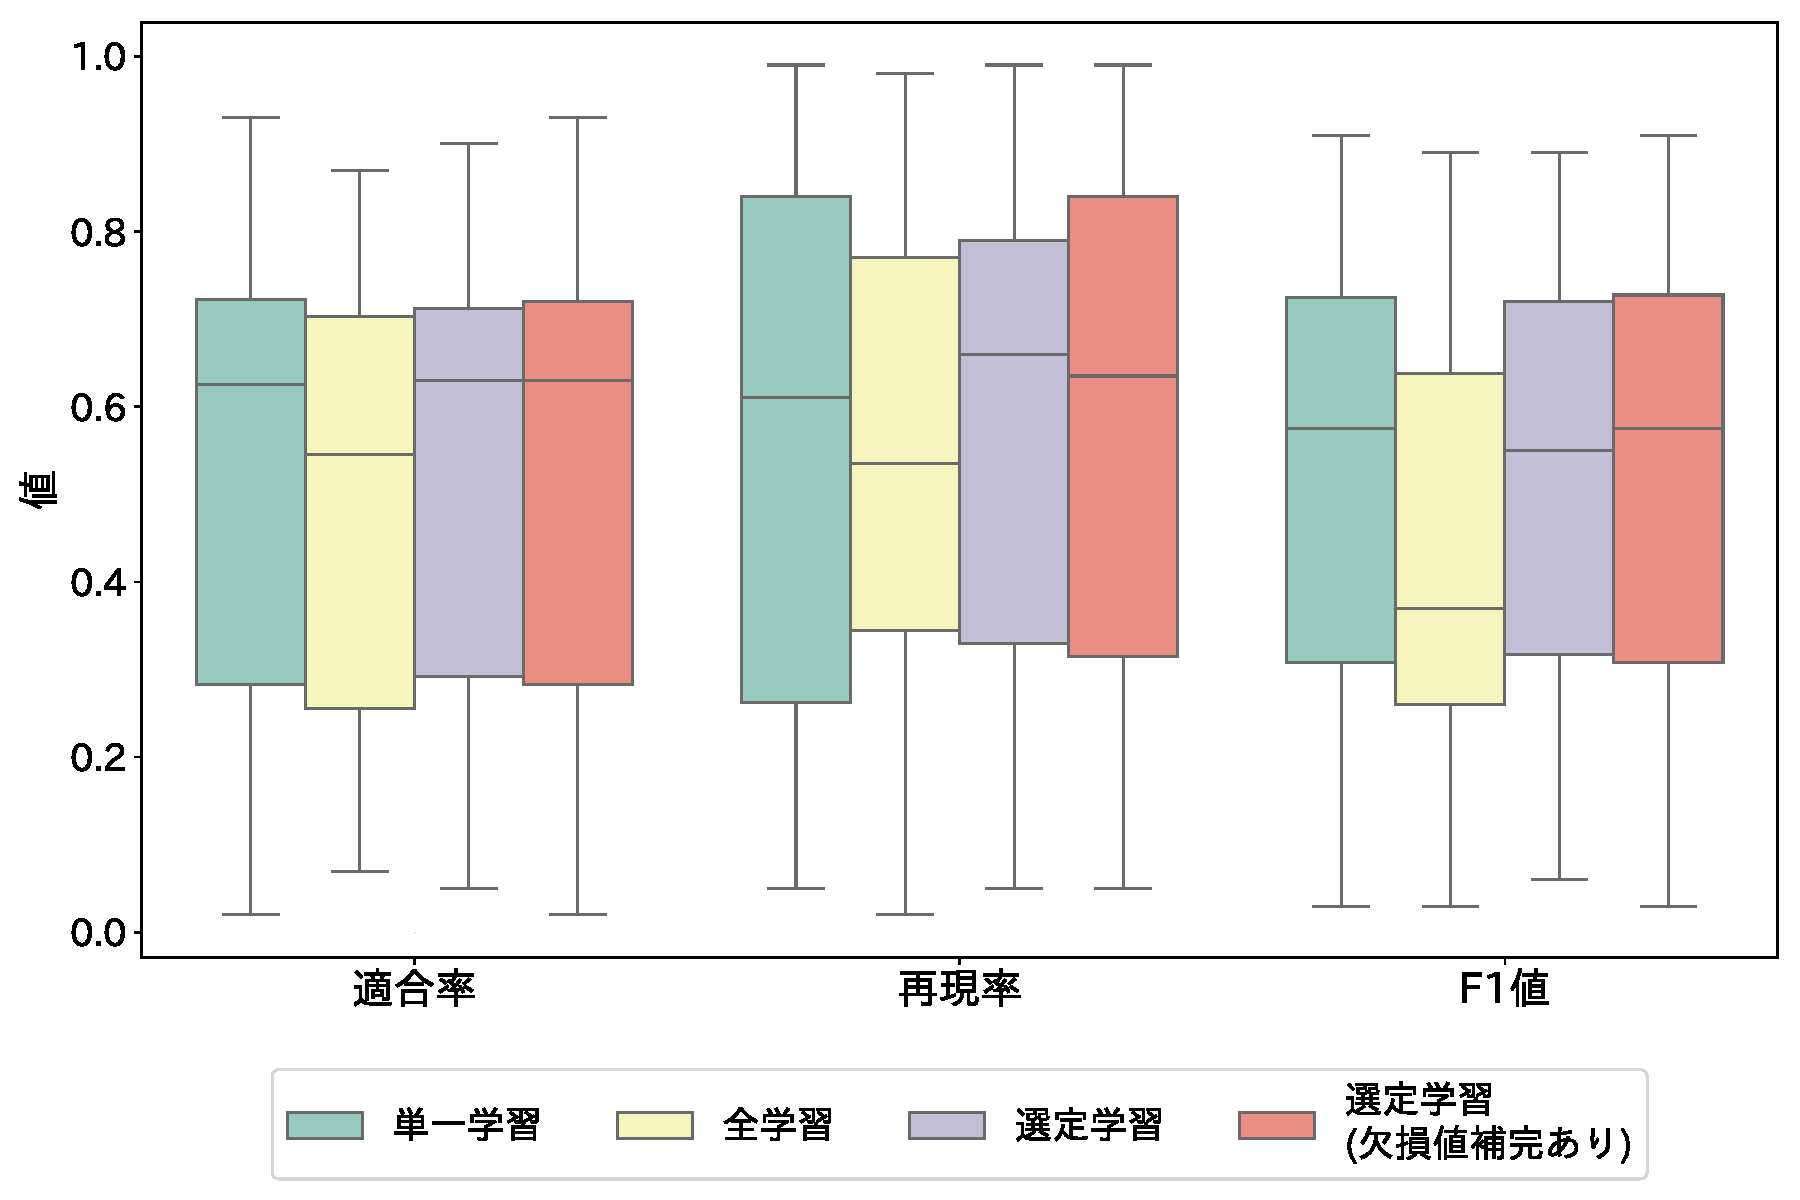
\includegraphics[width=1\linewidth]{fig/boxplot_unfiltered.pdf}
	\caption{4手法による予測結果の箱ひげ図}
	\label{fig:boxplot}
\end{figure}

\begin{figure}[t]
	\centering
        % 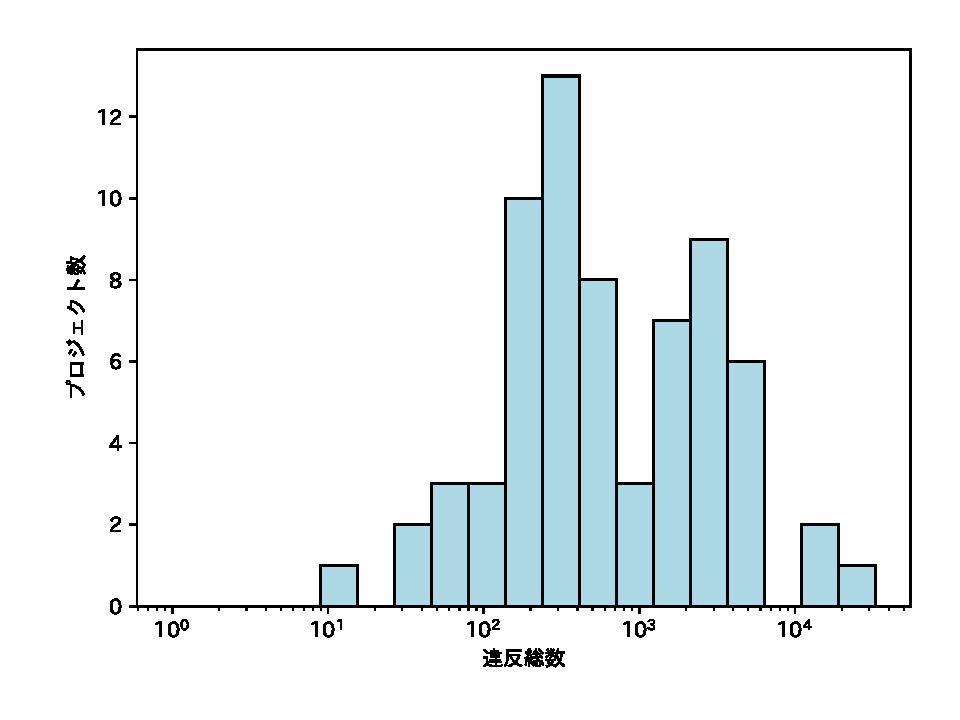
\includegraphics[width=0.25\textwidth, bb=0 0 4 3]{fig/dataset_hist.pdf}
	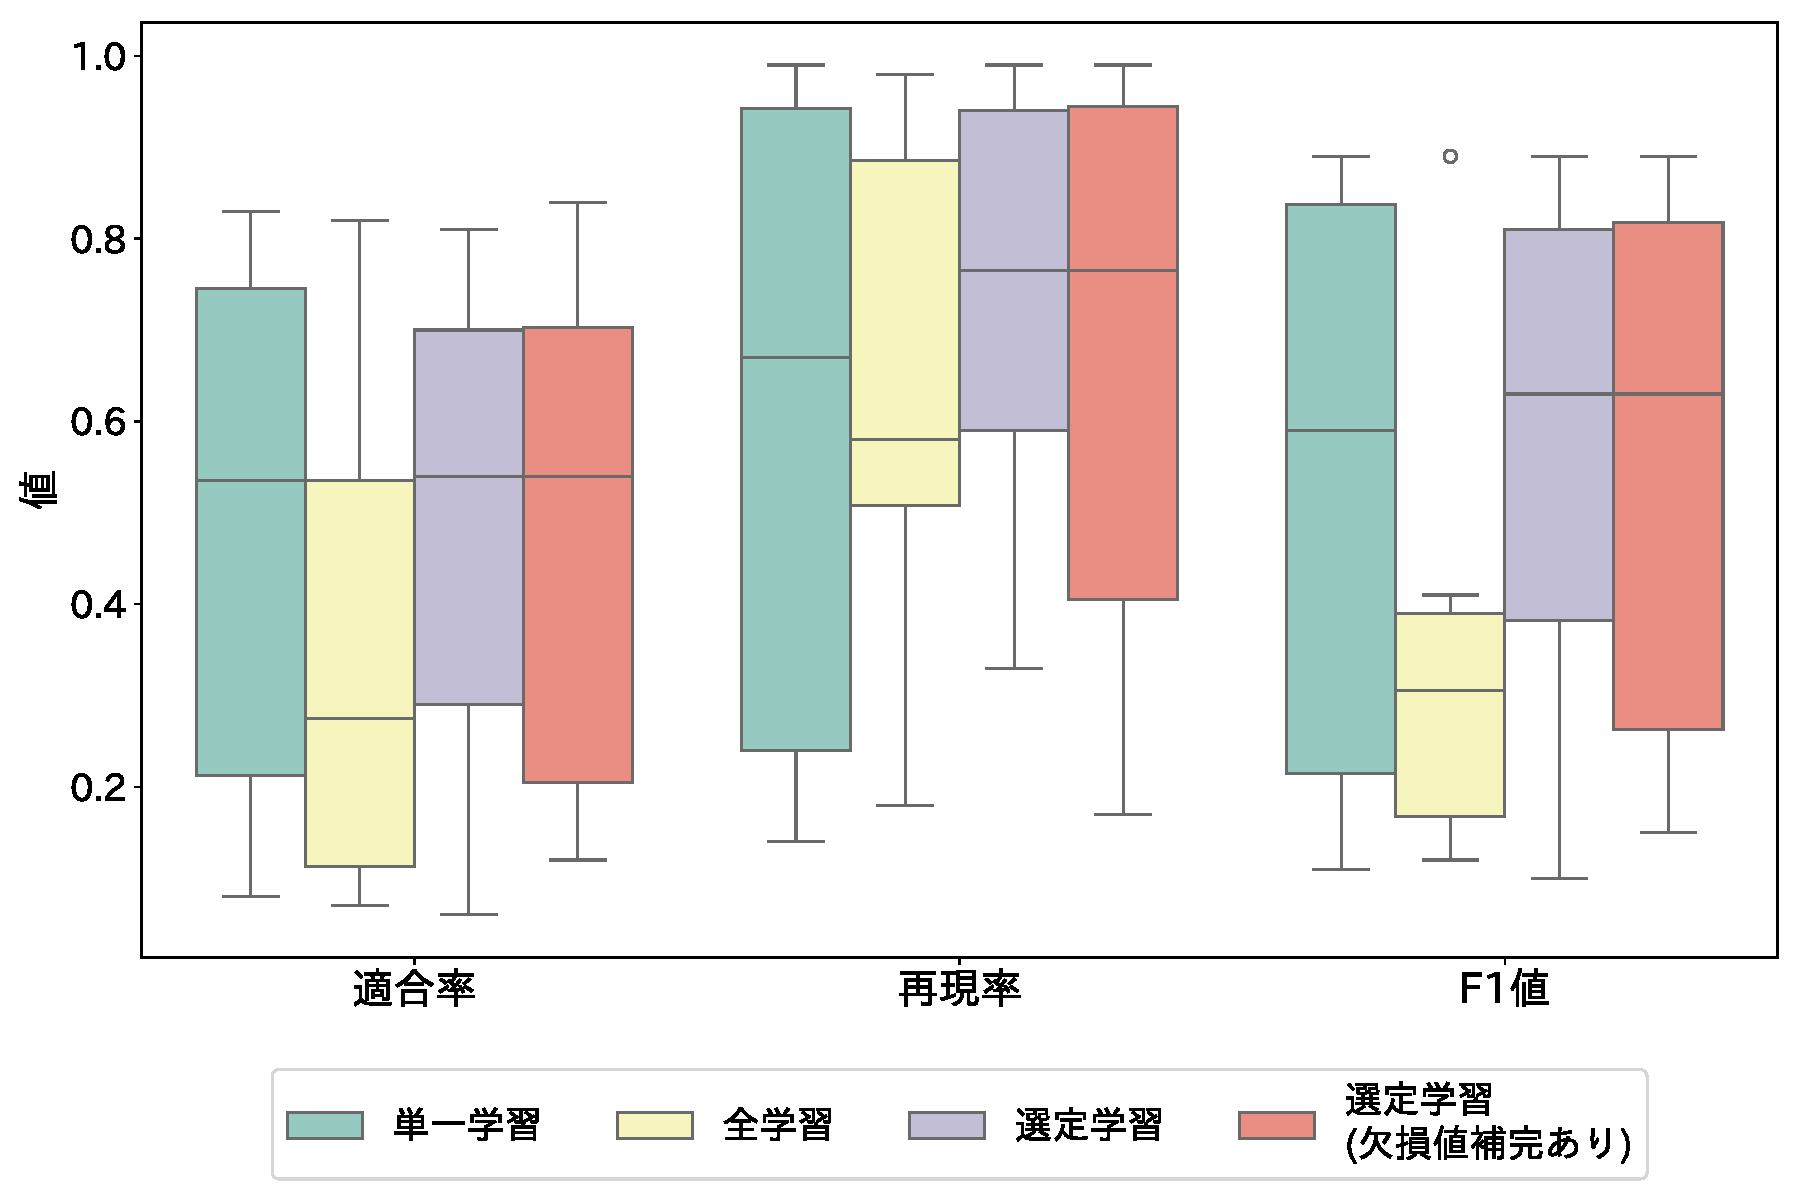
\includegraphics[width=1\linewidth]{fig/boxplot_filtered.pdf}
	\caption{選定学習手法(欠損値補完あり)で複数プロジェクトのデータを学習したプロジェクトに絞った予測結果の箱ひげ図}
	\label{fig:boxplot_filtered}
\end{figure}

表\ref{table:result1}に本研究の4種類の手法による予測結果の一覧を示す.
表の最初の列には予測対象プロジェクト名を示し,2列目以降にそれぞれの手法による適合率,再現率,F1値を示す.
図\ref{fig:boxplot}には,表\ref{table:result1}に示した結果を箱ひげ図で示す.
まず,表\ref{table:result1}から従来手法の単一学習と提案手法の全学習を比較すると,15プロジェクトにおいて単一学習の方がF1値が高い.図\ref{fig:boxplot}からも全学習のF1値が他手法に比べて低いことがわかる.
全学習により予測精度が低下する結果は,予測していた通りの結果である.
全学習による予測精度の低下は,コーディング規約違反の修正要否の予測にあたり,単に他プロジェクトのデータを学習に追加するだけでは予測精度が低下することを示している.

次に選定学習の結果について述べる.\ref{chap:選定方法}章において,選定学習におけるプロジェクト間類似度の測定方法について説明した.その最適な類似度測定の閾値について検証した結果は以下の通りである.
本研究で最も予測精度が高く出力された閾値は,選定学習では(ジャッカード係数:0.3以下,ユークリッド距離:3.0以下)であり,選定学習(欠損値補完あり)では(ジャッカード係数:0.3以下,ユークリッド距離:3.5以下)である.これらの閾値を採用し,類似プロジェクトの学習データの統合を行い,修正要否予測を行った結果を表\ref{table:result1}に示す.

図\ref{fig:boxplot}の選定学習の予測結果に注目すると,全学習の結果と比較して予測精度の改善が見られる.再現率の中央値に関しては,従来手法である単一学習からわずかに改善が見られる.
しかし,適合率とF1値に関しての予測精度の変化は見られない.

最後に選定学習(欠損値補完あり)の結果について述べる.図\ref{fig:boxplot}から,選定学習(欠損値補完あり)の結果は,欠損値補完を行わない選定学習手法から大きな変化がないことがわかる.この結果の要因として,選定学習(欠損値補完あり)において,複数プロジェクトの学習データを統合して学習していたプロジェクトが,6プロジェクトのみであることが要因の一つとして考えられる.
複数プロジェクトのデータを学習に利用していた,予測対象プロジェクトは表\ref{table:result1}のプロジェクト名に下線を引いている6プロジェクトである.
つまり,下線が引かれていない14プロジェクトでは,類似しているプロジェクトが無いという結果となり,予測対象プロジェクトの過去のデータのみを利用した単一学習と同じ結果となり,変化があまり見られない結果となっている.
そこで,選定学習(欠損値補完あり)において,複数プロジェクトの学習データを統合して学習していた6プロジェクトに絞り,予測結果を箱ひげ図にしたものを図\ref{fig:boxplot_filtered}に示す.
図\ref{fig:boxplot_filtered}から,欠損値補完の有無によらず,選定学習では,単一学習と比較して,適合率を維持した状態で,再現率が改善されている.また,再現率が向上したことによるF1値の向上も見られる.
また,再現率においては,全学習においても,中央値では単一学習より低下しているが,最小値や第一四分位数が改善している.

結論として,複数の学習データを統合することは,コーディング規約違反の修正要否予測において,再現率を向上させることが示唆される.ただし,全学習のようにプロジェクトの修正傾向を無視した単に学習データの統合を行うだけでは,適合率が大幅に低下し,F1値が低下してしまうため,予測精度を改善するためには統合するプロジェクトは選定する必要がある.

\subsection{予測性に改善が見られるプロジェクトに特徴はあるか?}

% sockeye: ['hickle', 'pyscard', 'transitions']
% coretools: ['hickle', 'pyscard']
% howdoi: ['pyscard']
% schema_salad: ['hickle', 'pyscard']
% serverless-application-model: ['OWSLib', 'pynput', 'schematics', 'hickle', 'python-sdk', 'datadogpy', 'pyscard', 'transitions']
% SoCo: ['pynput', 'schematics', 'hickle', 'python-sdk', 'GPflow', 'transitions', 'pyphi']
% behave: ['pynput', 'hickle']
% OWSLib: ['serverless-application-model', 'hickle', 'datadogpy', 'pyscard']
% pynput: ['serverless-application-model', 'SoCo', 'behave', 'schematics', 'hickle', 'python-sdk', 'datadogpy', 'GPflow', 'transitions', 'pyphi']
% schematics: ['serverless-application-model', 'SoCo', 'pynput', 'hickle', 'python-sdk', 'datadogpy', 'GPflow', 'pyphi']
% hickle: ['coretools', 'schema_salad', 'serverless-application-model', 'SoCo', 'behave', 'OWSLib', 'pynput', 'schematics', 'rtv', 'datadogpy', 'pyscard', 'GPflow', 'transitions', 'pyphi']
% python-sdk: ['serverless-application-model', 'SoCo', 'pynput', 'schematics', 'rtv', 'datadogpy', 'pychromecast', 'GPflow', 'transitions', 'pyphi']
% rtv: ['hickle', 'python-sdk']
% datadogpy: ['serverless-application-model', 'OWSLib', 'pynput', 'schematics', 'hickle', 'python-sdk', 'pyscard']
% pychromecast: ['python-sdk', 'GPflow']
% pyscard: ['coretools', 'howdoi', 'schema_salad', 'serverless-application-model', 'OWSLib', 'hickle', 'datadogpy']
% GPflow: ['SoCo', 'pynput', 'schematics', 'hickle', 'python-sdk', 'pychromecast', 'transitions']
% transitions: ['serverless-application-model', 'SoCo', 'pynput', 'hickle', 'python-sdk', 'GPflow', 'pyphi']

% === coretools (RandomForest) の重要度上位10カラム ===
%  1. AvgLineBlank                   0.0452
%  2. CountLineBlank                 0.0352
%  3. CountLine                      0.0331
%  4. CountLineComment               0.0326
%  5. CountLineCode                  0.0300
%  6. CountStmt                      0.0278
%  7. CountLineCodeExe               0.0269
%  8. RatioCommentToCode             0.0260
%  9. E0401                          0.0247
% 10. CountStmtExe                   0.0237

% === behave (RandomForest) の重要度上位10カラム ===
%  1. CountLineCode                  0.0528
%  2. CountStmt                      0.0525
%  3. CountLineCodeExe               0.0480
%  4. CountStmtDecl                  0.0460
%  5. AvgLine                        0.0451
%  6. CountLineCodeDecl              0.0443
%  7. W1406                          0.0408
%  8. CountLine                      0.0408
%  9. CountStmtExe                   0.0321
% 10. C0209                          0.0287

% === hickle (RandomForest) の重要度上位10カラム ===
%  1. W0612                          0.0786
%  2. CountLine                      0.0781
%  3. CountLineBlank                 0.0739
%  4. C0209                          0.0547
%  5. C0116                          0.0536
%  6. CountDeclMethodAll             0.0478
%  7. C0305                          0.0298
%  8. E0401                          0.0279
%  9. E0602                          0.0279
% 10. CountStmtExe                   0.0250

% === python-sdk (RandomForest) の重要度上位10カラム ===
%  1. C0209                          0.1187
%  2. R0205                          0.1034
%  3. CountLineCode                  0.0353
%  4. RatioCommentToCode             0.0337
%  5. CountLineCodeExe               0.0335
%  6. CountLine                      0.0321
%  7. CountStmt                      0.0293
%  8. CountLineComment               0.0286
%  9. CountLineCodeDecl              0.0278
% 10. CountStmtExe                   0.0261

% === pyscard (RandomForest) の重要度上位10カラム ===
%  1. E0001                          0.1129
%  2. E0602                          0.0486
%  3. C0121                          0.0449
%  4. AvgLineCode                    0.0431
%  5. C0103                          0.0415
%  6. CountLineCodeDecl              0.0260
%  7. AvgLine                        0.0237
%  8. RatioCommentToCode             0.0232
%  9. CountLineComment               0.0223
% 10. CountLine                      0.0222

% === datadogpy (RandomForest) の重要度上位10カラム ===
%  1. CountLineCodeExe               0.0453
%  2. CountLineCode                  0.0420
%  3. CountStmtExe                   0.0398
%  4. C0301                          0.0396
%  5. RatioCommentToCode             0.0362
%  6. CountLine                      0.0339
%  7. CountStmt                      0.0339
%  8. CountLineBlank                 0.0291
%  9. CountLineComment               0.0258
% 10. C0209                          0.0255

% === howdoi (RandomForest) の重要度上位10カラム ===
%  1. CountLineCodeExe               0.1246
%  2. CountStmtExe                   0.1021
%  3. CountLine                      0.0924
%  4. CountLineCode                  0.0891
%  5. CyclomaticModified             0.0676
%  6. RatioCommentToCode             0.0568
%  7. Essential                      0.0521
%  8. CountClassBase                 0.0484
%  9. Cyclomatic                     0.0447
% 10. CyclomaticStrict               0.0407

% === rtv (RandomForest) の重要度上位10カラム ===
%  1. C0209                          0.0569
%  2. E0401                          0.0400
%  3. CountLineCodeExe               0.0317
%  4. R0914                          0.0301
%  5. R0915                          0.0290
%  6. CountStmt                      0.0276
%  7. CountLine                      0.0271
%  8. CountLineCode                  0.0266
%  9. CountStmtExe                   0.0266
% 10. R1705                          0.0253



% === GPflow (RandomForest) の重要度上位10カラム ===
%  1. C0301                          0.0539
%  2. CountLineCode                  0.0511
%  3. CountLine                      0.0449
%  4. E0401                          0.0436
%  5. C0305                          0.0393
%  6. E0602                          0.0376
%  7. CountStmt                      0.0374
%  8. W0611                          0.0365
%  9. CountLineBlank                 0.0357
% 10. RatioCommentToCode             0.0331

% === transitions (RandomForest) の重要度上位10カラム ===
%  1. C0209                          0.0982
%  2. CountLine                      0.0353
%  3. CountLineCodeExe               0.0347
%  4. CountStmt                      0.0326
%  5. CountLineCode                  0.0319
%  6. SumCyclomaticModified          0.0313
%  7. C0103                          0.0308
%  8. C0411                          0.0300
%  9. CountLineCodeDecl              0.0299
% 10. CountStmtExe                   0.0295

\begin{figure}[t]
	\centering
        % 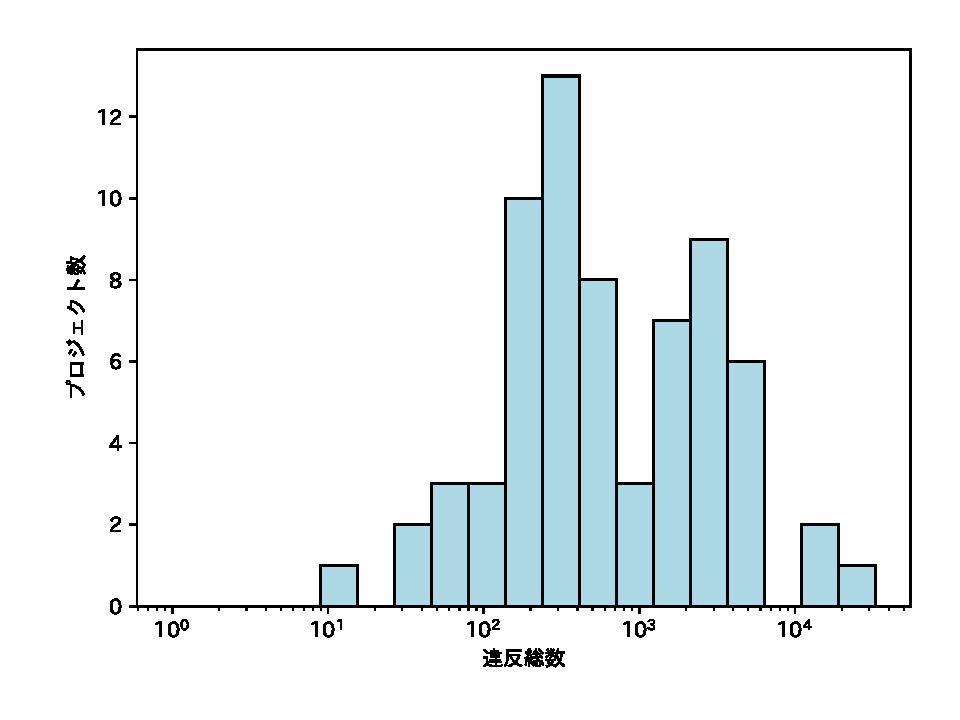
\includegraphics[width=0.25\textwidth, bb=0 0 4 3]{fig/dataset_hist.pdf}
	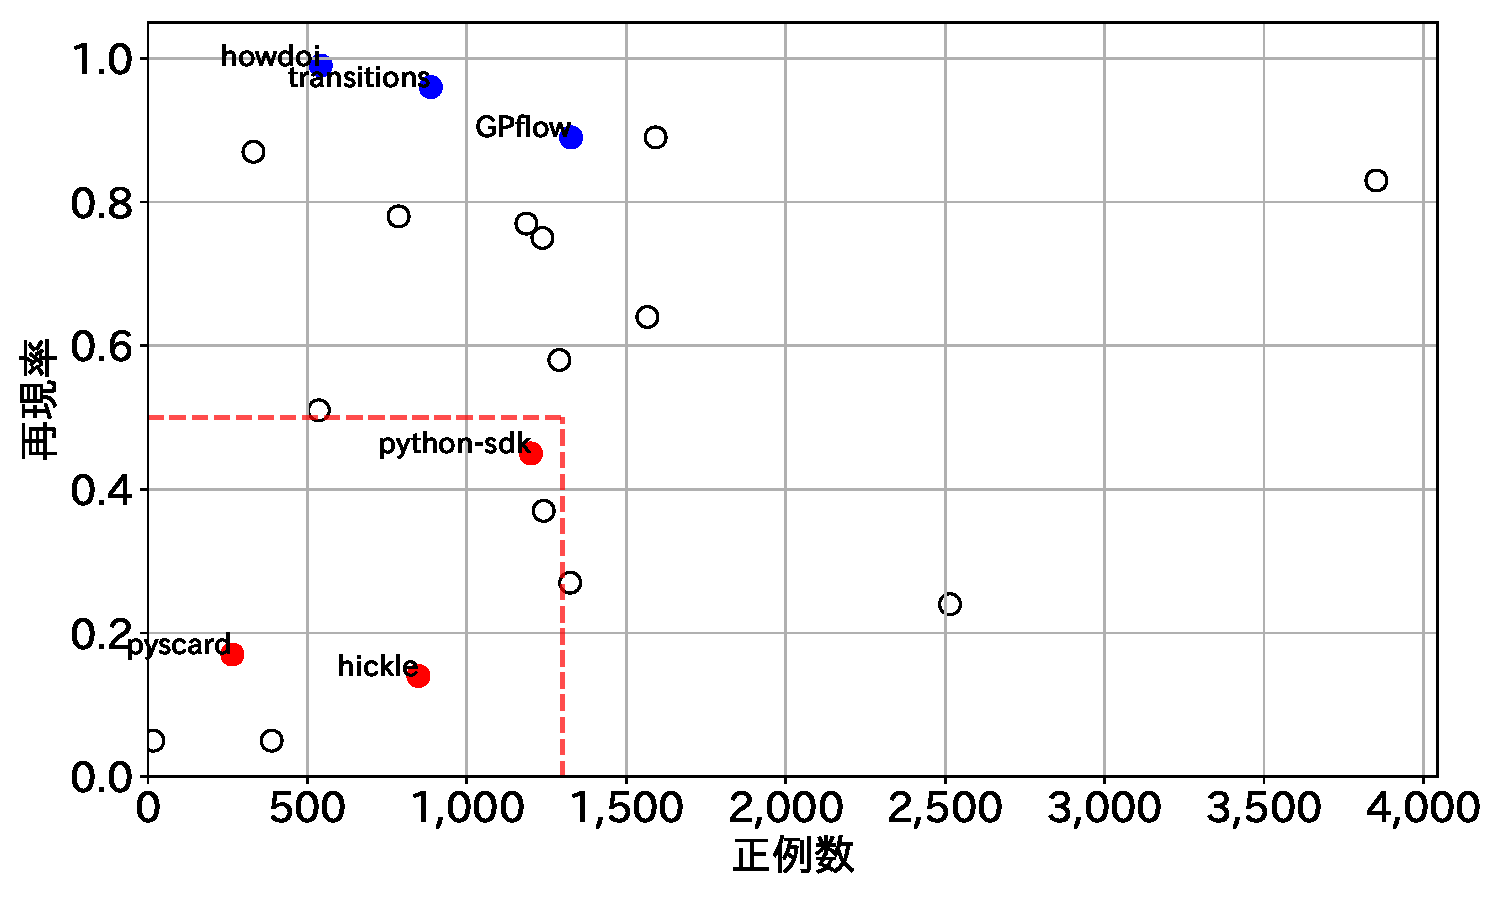
\includegraphics[width=1\linewidth]{fig/sannpuzu.pdf}
	\caption{正例数と単一学習の再現率の散布図}
	\label{fig:scatter_plot_filtered}
\end{figure}

結果から,類似プロジェクトの学習データの統合によって,再現率が向上することが示唆された.
本節では,この再現率向上が見られるプロジェクトの共通点を分析する.
図\ref{fig:scatter_plot_filtered}は,プロジェクトの学習データにおける正例数を横軸に,単一学習の再現率を縦軸にとった散布図である.選定学習(欠損値補完あり)において複数プロジェクトの学習データを統合して学習した6プロジェクトは,プロットに色とプロジェクト名を付与した.このうち,再現率が10ポイント以上向上したプロジェクトは赤色,それ以外のプロジェクトは青色で示されている.

4つの手法を比較するため,複数プロジェクトを学習したプロジェクトに着目して分析を進める.単一学習の再現率とデータセットの正例数には,弱い相関(0.35)が見られた.特に,正例数が400以下のプロジェクトでは予測精度がばらついている.

選定学習によって再現率が向上した3プロジェクトは,単一学習の再現率が0.5未満に集中していた.一方,再現率が低下または同程度だった3プロジェクトは,単一学習の再現率が0.8以上に集中している.
この6プロジェクトの分析から,選定学習によって再現率が向上するプロジェクトには,以下の2つの共通点があることが明らかになった.
\begin{enumerate}
    \item データセット内の正例数が1,300以下.
    \item 単一学習での再現率が0.5以下.
\end{enumerate}
これらの特徴は,特に選定学習(欠損値補完あり)で学習データを統合したプロジェクトにおいて顕著である.

欠損値補完を行わない選定学習では,上記の6プロジェクト以外にも学習データを統合したプロジェクトが存在するため,それらのプロジェクトについても分析を行った.
上記の2つの共通点に合致する,または概ね条件を満たしているプロジェクトは,選定学習(欠損値補完あり)で再現率が向上した3プロジェクト以外に,さらに5プロジェクト存在した.このうち1プロジェクトは類似プロジェクトが存在せず,単一学習と同様の結果であったため除外した.残る4プロジェクト(serverless-application-model,behave,rtv,datadogpy)について表\ref{table:result1}を用いて分析した結果,behaveプロジェクトを除く3プロジェクトでは,選定学習によって変化がないか,再現率が上昇していることが確認された.

総合すると,選定学習によって再現率が向上する上記の2条件を概ね満たすプロジェクトは,選定学習を適用した場合に7プロジェクト中5プロジェクトで再現率の上昇が見られた.
このことから,「データセット内の正例数が1,300以下」および「単一学習での再現率が0.5以下」という2つの条件を満たすことが,複数プロジェクトの学習データを統合することによる恩恵を受けるプロジェクトの有効な特徴であると強く示唆される.


%%%%%%%%%%%%%%%%%%%%%%%%%%%
\section{考察}\label{chap:consideration}
%%%%%%%%%%%%%%%%%%%%%%%%%%%

\subsection{学習データを統合することによって再現率が向上した要因}

結果として,複数プロジェクトの学習データを統合することで再現率が向上することが示唆された.学習データ統合によって再現率が向上した要因の一つとして,他プロジェクトから正例が補完されたことにより,予測できる正例の範囲が拡大したことが考えられる.

本研究では,学習データのスパース性に対応するため,学習時に正例データへ重みづけを行っている.そのため,補完される正例データが少数であっても,モデルへ大きな影響を与える.これにより,学習データの統合が再現率向上に繋がったと考えられる.

また,全学習で適合率が大幅に低下した要因についても,同様のメカニズムが考えられる.予測対象プロジェクトでは正例としない事象が,他プロジェクトでは正例として扱われていた場合,その数が少量であってもモデルが誤って正例と分類する要因となり,適合率の低下を招いた可能性がある.


\subsection{再現率が向上する条件に一致するが,再現率が低下したプロジェクトの要因}

\begin{figure}[t]
	\centering
        % 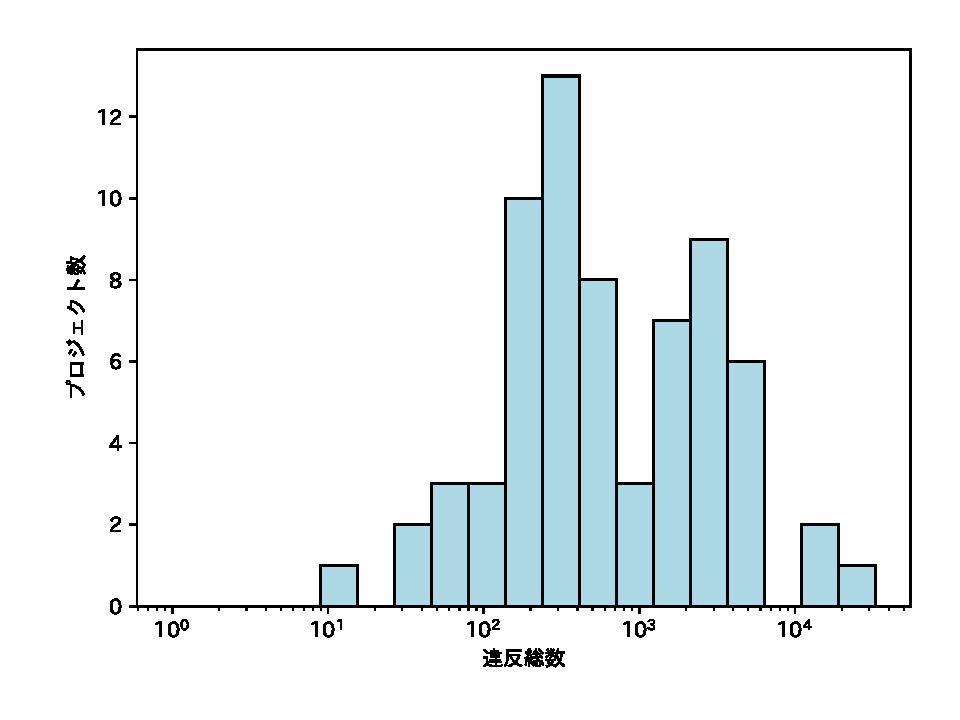
\includegraphics[width=0.25\textwidth, bb=0 0 4 3]{fig/dataset_hist.pdf}
	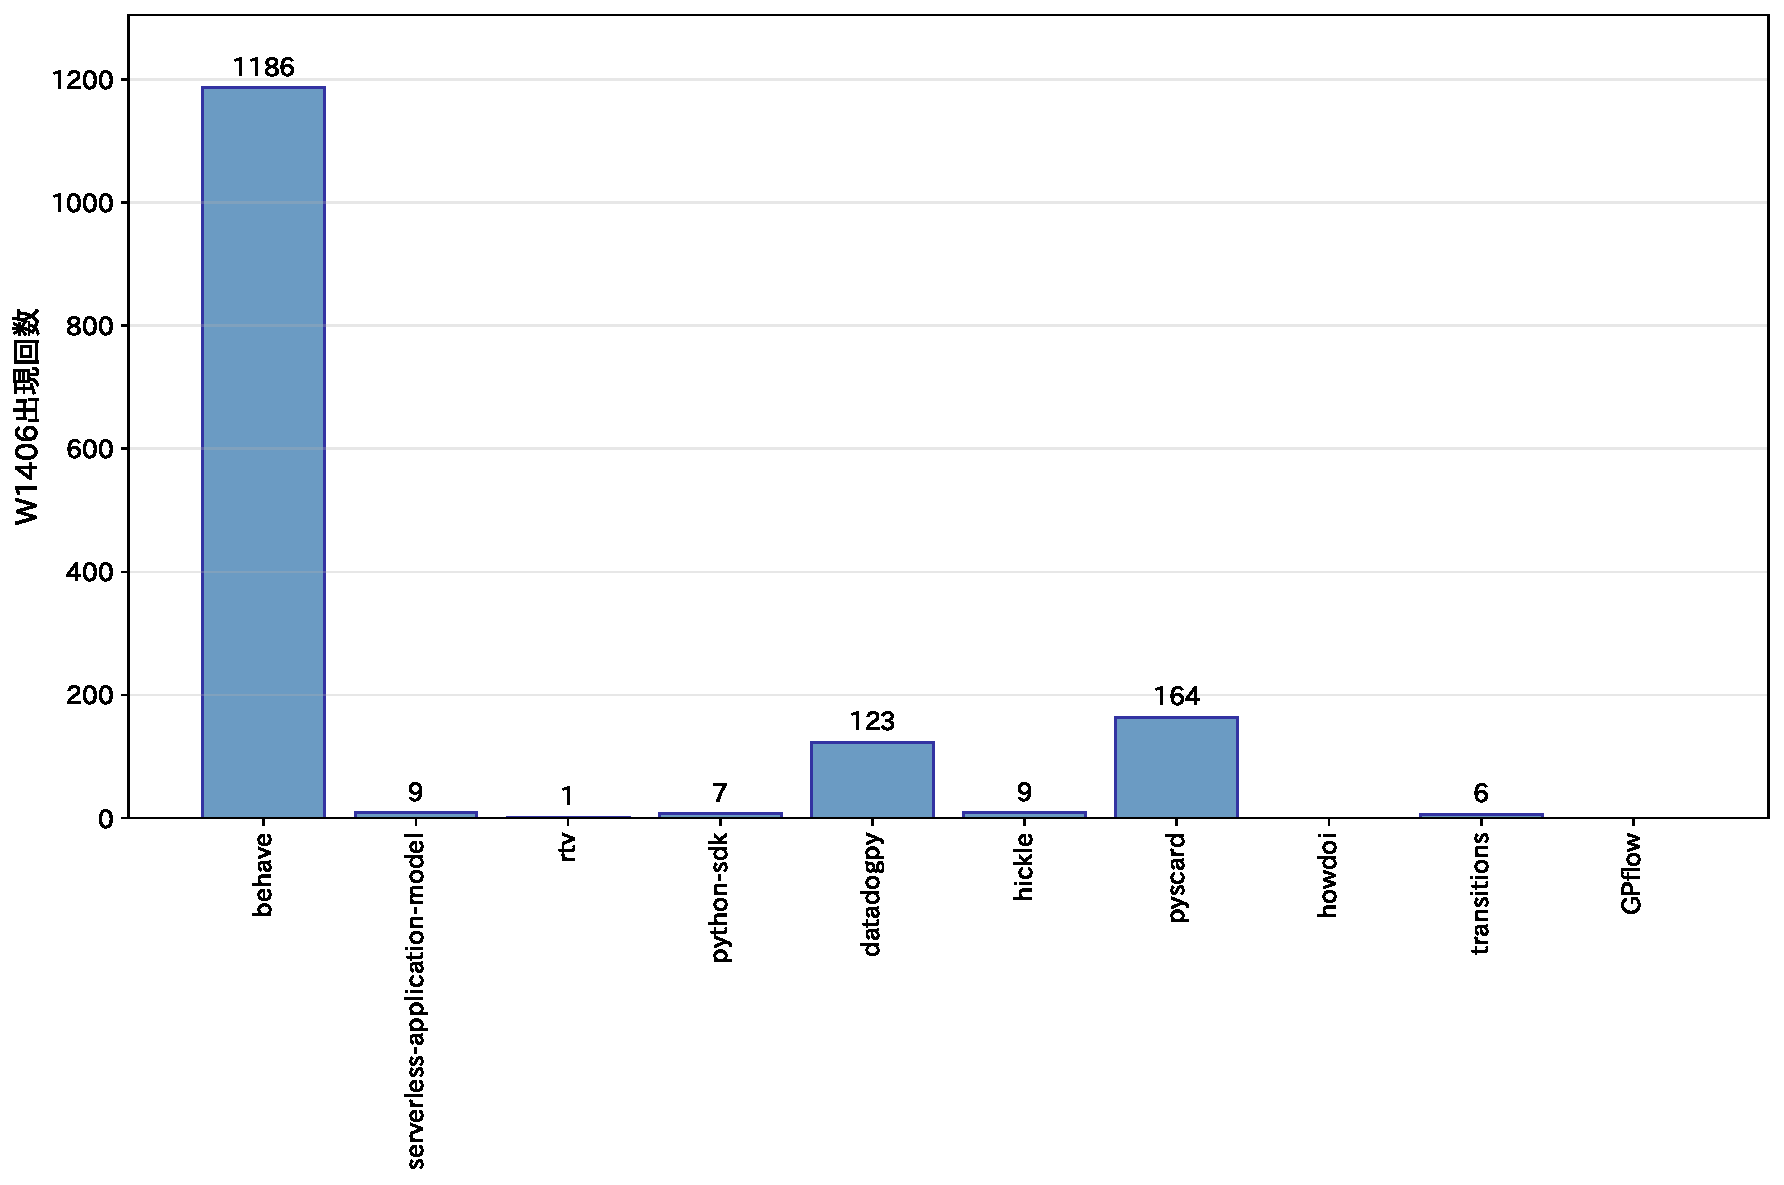
\includegraphics[width=1\linewidth]{fig/w1406_project_comparison.pdf}
	\caption{W1406のプロジェクト別出現頻度}
	\label{fig:w1406}
\end{figure}

behaveプロジェクトは,再現率が向上するプロジェクトの条件を概ね満たしていたにもかかわらず,選定学習によって再現率が13ポイント低下した.本節ではその要因を考察する.

behaveプロジェクトにおけるコーディング規約違反のデータ総数は3,549件であり,そのうち1,186件がW1406という種類のコーディング規約違反であった.これはプロジェクト全体の33\%を占める割合であり,選定学習によって再現率が低下しなかった他の6プロジェクトと比較すると,W1406の出現頻度におけるZスコアは6.95に達する.このことから,W1406がbehaveプロジェクトを象徴するコーディング規約違反であることがわかる.

図\ref{fig:w1406}に示すように,プロジェクトを象徴する特定のコーディング規約が存在する現象は,他のプロジェクトでも同様に見られる.しかし,他のプロジェクトでは,象徴的なコーディング規約の種類が「共通して発生しやすいもの」であるか,または「修正率が低い(正例数が少ないため再現率に影響しにくい)もの」であることが共通している.

一方,behaveプロジェクトを象徴するW1406の修正率は52\%であった.これは,プロジェクト内で当該規約が修正されるか否かの統一された方針が不明確であることを示唆する.さらに,予測精度が向上している他のプロジェクトでは,象徴的なコーディング規約が機械学習モデルの重要度の高い上位10件に含まれる傾向が見られたが,behaveプロジェクトではこの傾向は確認されなかった.

以上の分析から,本研究で提案する選定学習において,他のプロジェクトでは出現頻度の低いコーディング規約が特定のプロジェクト(behave)を象徴する規約となった場合,他のプロジェクトのデータを統合すると,当該プロジェクトを象徴していたコーディング規約の重要度が相対的に低下し,結果として再現率が低下したと考えられる.

%%%%%%%%%%%%%%%%%%%%%%%%%%%
\section{妥当性への脅威}\label{chap:heuristic}
%%%%%%%%%%%%%%%%%%%%%%%%%%%
\subsection{内的妥当性}


目的変数の計測において,規約違反しているコードが修正された場合のみ正例として扱い,削除された場合は,修正されたわけではないため本研究では負例として扱っている.しかし,コーディング規約違反の中には該当部分を削除することによっても解消するものがあるため,本来正例として扱うべきケースを負例として計測してしまっていることがある.
コードの移動に関してもGitHubの仕様上,削除と追加という扱いになるため,コードの移動によってコーディング規約に違反しているコードが削除され不例として計測している可能性がある.
% また,コーディング規約に違反しているコードが,可読性とは関係のない実行速度などの観点からコードが修正された場合でも,違反していたコードが削除された場合は不例として計測してしまっている.


% 本研究で用いた2種類の機械学習アルゴリズム以外にも,より正確な予測を可能にするアルゴリズムが存在する可能性がある.
% それぞれのパラメータの更新回数である,イテレーション回数を10,000に設定したが,データサイズが大きいプロジェクトではモデルが収束しないことが確認された.モデルが収束しない場面も確認されたが,本研究で主に用いた実験環境とは別の環境で,複数回実行した場合でも予測結果に変化はなかったので,モデルが収束しない問題に関しては,本研究の結果に対して大きな影響を与える可能性は低い.


\subsection{外的妥当性}

本研究ではケーススタディとしてPython言語を主な開発言語としたプロジェクト20件の規約違反修正履歴を収集して検証を行った.
また,プロジェクト数をさらに拡張した場合や,対象とするプロジェクトや期間を変更した場合に予測精度が変化することが示唆される.
対象言語をPython以外の言語とした場合予測結果が変化することが示唆される.
しかし,本研究で利用したデータセットは,データ数の平均値が4,465であり,十分なデータ数を確保できているため,データ数を各量することによる予測精度の低下の可能性は低いと考えられる.また,選定学習においては,より類似度の高いプロジェクトを統合できるため,更なる予測精度の向上が見込める.

%%%%%%%%%%%%%%%%%%%%%%%%%%%
\section{おわりに}\label{chap:end}
%%%%%%%%%%%%%%%%%%%%%%%%%%%

本研究では,静的解析ツールによってソースコード中に含まれるコーディング規約違反を検出した結果から,修正すべき違反か否かに分類するタスクにおいて,予測対象プロジェクト以外の開発データも予測モデルの学習に用いた場合の予測結果への影響を調査した.

結果として,予測対象プロジェクト以外の開発データも学習する提案手法によって,検証に使用した20プロジェクトの内,特定の条件を満たす7プロジェクトのうち5プロジェクトで再現率の向上が見られた.再現率が低下したプロジェクトにおいては,発生しているコーディング規約違反の傾向が他プロジェクトと大きく異なる,特殊なデータであった.このことから,条件を満たすプロジェクトであれば,概ね提案手法である選定学習によって再現率の上昇が見込める.

再現率が上昇する理由としては,修正する必要があると判断する正例データが基本的に負例に比べて少ないため,正例データを他プロジェクトからも学習することで,モデルがより多くの修正すべき違反を識別できるようになり,再現率が上昇したと考えられる.

本研究において,選定学習により再現率が向上するプロジェクトの条件が明らかになった.この条件を満たすプロジェクトのデータを拡張して収集し,より類似度の高いプロジェクトのデータを学習することで,単一学習では再現率が低いプロジェクトにおいて,さらなる再現率の向上が見込める.

% \ack %% 謝辞

%\bibliographystyle{sieicej}
%\bibliography{myrefs}
\bibliographystyle{sieicej}
\bibliography{Kameoka}
% \begin{thebibliography}{99}% 文献数が10未満の時 {9}
% \bibitem{}
% \end{thebibliography}

% \appendix
% \section{}

%% 著者紹介・顔写真の掲載はC分冊の場合は任意です.
\begin{biography}
\profile{n}{亀岡 令}{サンプル}
%\profile{会員種別}{名前}{紹介文}% 顔写真あり
%\profile*{会員種別}{名前}{紹介文}% 顔写真なし
\end{biography}

\end{document}
